%% LyX 2.3.0rc2 created this file.  For more info, see http://www.lyx.org/.
%% Do not edit unless you really know what you are doing.
\documentclass[dutch]{scrartcl}
\usepackage[T1]{fontenc}
\usepackage[latin9]{inputenc}
\usepackage{geometry}
\geometry{verbose,tmargin=2.5cm,bmargin=2.5cm,lmargin=2.5cm,rmargin=2.5cm}
\usepackage{color}
\usepackage{array}
\usepackage{float}
\usepackage{url}
\usepackage{stmaryrd}
\usepackage{graphicx}

\makeatletter

%%%%%%%%%%%%%%%%%%%%%%%%%%%%%% LyX specific LaTeX commands.
%% Because html converters don't know tabularnewline
\providecommand{\tabularnewline}{\\}

\makeatother

\usepackage{babel}
\begin{document}

\title{Handleiding V\&A in Zotero/Juris-M}

\author{Mathijs van Westendorp\thanks{Email: mathijs.vanwestendorp@kuleuven.be} }

\maketitle
Doordat de stylesheet nog niet grondig getest is, is het mogelijk
dat velden nog van betekenis veranderen. Daardoor is het mogelijk
dat latere versies niet meer dezelfde velden gebruiken en de items
in Zotero/Juris-M moeten worden aangepast. \textbf{\textsc{\textcolor{red}{De
veldkeuze is dus nog niet gefinaliseerd!!!}}}

\section{Installatie}

\subsection{Installeer Zotero of Juris-M}

Juris-M is een Zotero variant toegespitst op juridisch verwijzen.
Dit voegt ondersteuning toe voor zaken als Kamerstukken, wetten en
jurisprudentie.

Om naar die zaken te kunnen verwijzen is dus Juris-M nodig. De bibliotheken,
instellingen etc. uit Zotero zijn compatibel met Juris-M.

Zie: \url{https://juris-m.github.io/downloads/}

\subsection{Installeer Stylesheet}

Toevoegen van Stylesheet in Zotero/Juris-M: Bewerken \ensuremath{\rightarrowtriangle}
Citeren \ensuremath{\rightarrowtriangle} 
\includegraphics{v-en-a/Manual-plus-sign}

\begin{figure}[H]
\begin{centering}
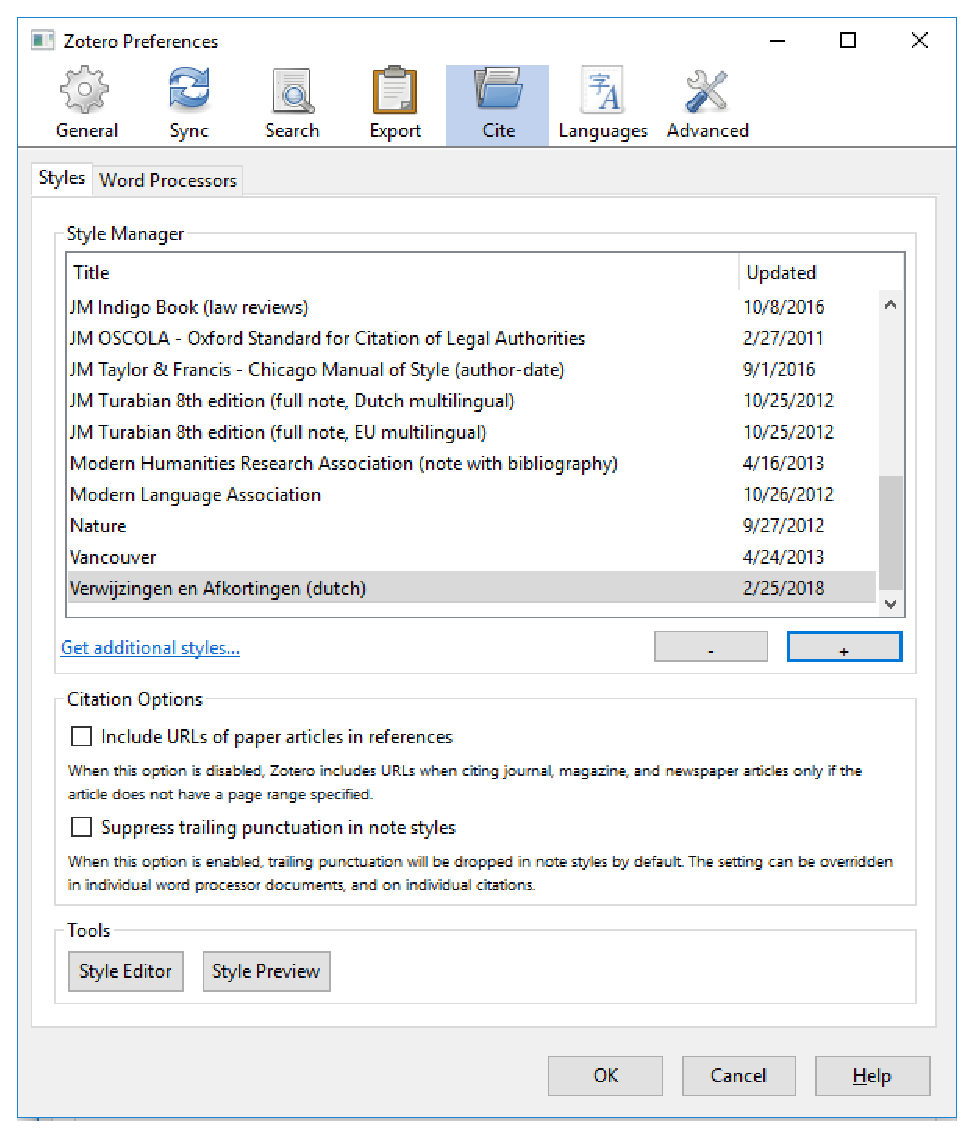
\includegraphics[scale=0.5]{v-en-a/Manual-fig-1}
\par\end{centering}
\caption{Toevoegen Stylesheet}
\end{figure}

! In Zotero geeft dit een waarschuwing dat het Stylesheet niet aan
de csl 1.0.1 voldoet, dit is omdat de extra opties voor Juris-M zijn
toegevoegd

\pagebreak{}

\section{Toevoegen aan de bibliotheek}

\subsection{Kamerstukken}

\textit{Hand}. Kamer 1989-90, 23 mei 1990, 68--79.

\begin{table}[H]
\begin{centering}
\begin{tabular*}{1\textwidth}{@{\extracolsep{\fill}}|>{\centering}p{0.15\textwidth}|>{\centering}p{0.3\textwidth}|>{\centering}p{0.3\textwidth}|}
\hline 
Veld & Soort waarde & Voorbeeld\tabularnewline
\hline 
\hline 
Type Item & 'Kamerstukken / Handelingen / Wetsvoorstel' & \tabularnewline
\hline 
Jurisdiction & Belgium|BE & \tabularnewline
\hline 
(Wetgevend) orgaan & Tekst + datum & Kamer 1989-90\tabularnewline
\hline 
Session Type & Afkorting zoals opgenomen in V\&A & Hand. ; Parl. St ; Vr. en Antw.\tabularnewline
\hline 
Datum & een geldige datum & 23 mei 1990\tabularnewline
\hline 
Sectie & Getal & 309\tabularnewline
\hline 
Pagina's & Relevante pagina's & 68-79\tabularnewline
\hline 
\end{tabular*}
\par\end{centering}
\caption{Kamerstukken / Handelingen / Wetsvoorstel}
\end{table}

\begin{figure}[H]
\begin{centering}
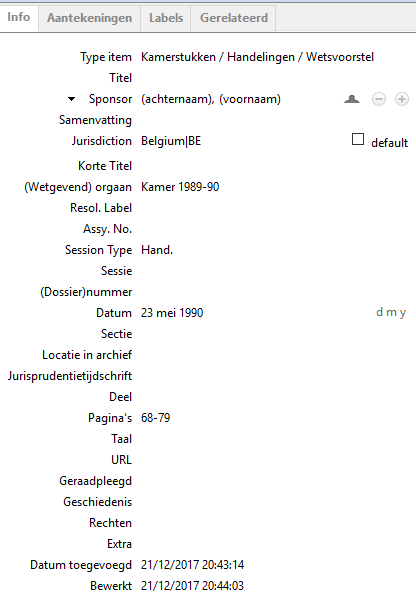
\includegraphics[scale=0.5]{v-en-a/Manual-fig-2}
\par\end{centering}
\caption{Kamerstukken weergave in Juris-M}
\end{figure}

\pagebreak{}

\subsection{Wet}

Wet van 6 juli 2007 betreffende de medisch begeleide voortplanting
en de bestemming van de overtallige embryo\textquoteright s en de
gameten, \textit{BS} 17 juli 2007 (Wet Medisch Begeleide Voortplanting).

\begin{table}[H]
\begin{tabular*}{1\textwidth}{@{\extracolsep{\fill}}|c|>{\centering}p{0.3\textwidth}|>{\centering}p{0.4\textwidth}|}
\hline 
Veld & Soort waarde & Voorbeeld\tabularnewline
\hline 
\hline 
Type Item & Wet & \tabularnewline
\hline 
Jurisdiction & Belgium|BE & \tabularnewline
\hline 
Citeertitel wet & Tekst & Wet van 6 juli 2007 betreffende de medisch begeleide voortplanting
en de bestemming van de overtallige embryo\textquoteright s en de
gameten\tabularnewline
\hline 
Korte Titel & Korte tekst & \multicolumn{1}{c|}{Wet Medisch Begeleide Voortplanting}\tabularnewline
\hline 
Publicatiemedium & Tekst & \multicolumn{1}{c|}{BS}\tabularnewline
\hline 
Datum publicatie & Datum & 17 juli 2007\tabularnewline
\hline 
\end{tabular*}

\caption{Wet}
\end{table}

\begin{figure}[H]
\begin{centering}
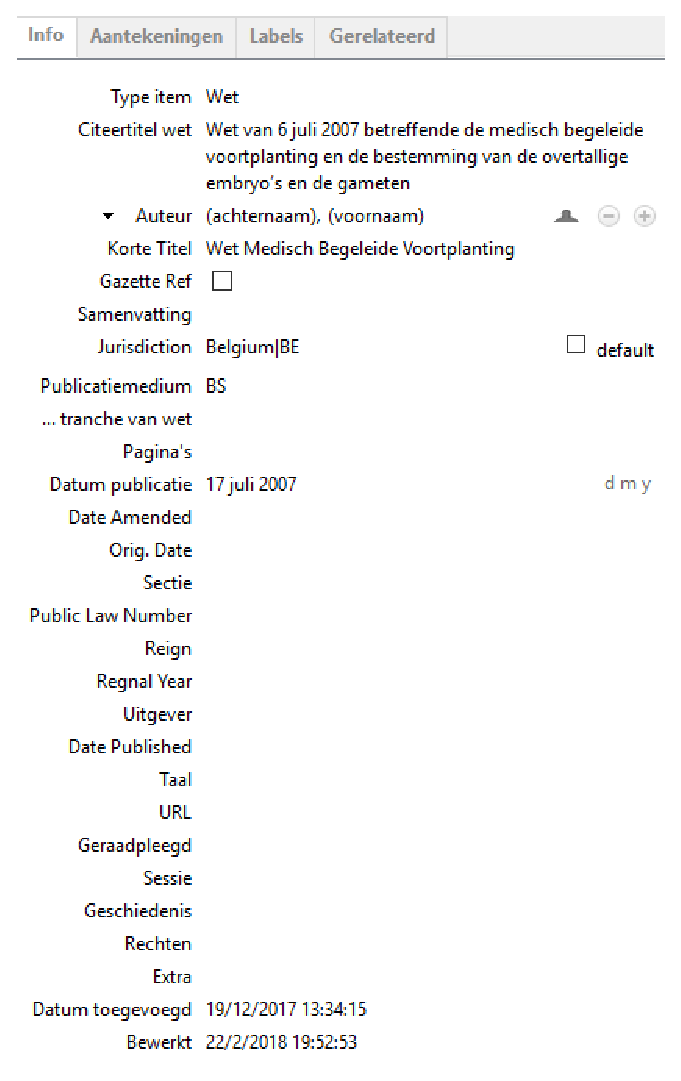
\includegraphics[scale=0.5]{v-en-a/Manual-fig-3}
\par\end{centering}
\caption{Wet weergave in Juris-M}
\end{figure}

\pagebreak{}

\subsection{Rechtspraak}

Cass. 27 januari 2011, \textit{TBH} 2011, 651, concl. A. HENKES, noot
R. HOUBEN.

\begin{table}[H]
\begin{tabular*}{1\textwidth}{@{\extracolsep{\fill}}|>{\centering}p{0.2\textwidth}|>{\centering}p{0.4\textwidth}|>{\centering}p{0.2\textwidth}|}
\hline 
Veld & Soort waarde & Voorbeeld\tabularnewline
\hline 
\hline 
Type Item & Rechtszaak & \tabularnewline
\hline 
Jurisdiction & Belgium|BE & \tabularnewline
\hline 
Naam rechtszaak & Tekst in Zotero/Juris-M & X en Y\tabularnewline
\hline 
Commentator & By auteur te vinden & A. Henkes\tabularnewline
\hline 
Korte Titel & Naam waaronder zaak bekend staat & \tabularnewline
\hline 
Rechtbank & Afkorting van de rechtbank & Cass.\tabularnewline
\hline 
Datum beslissing & Geldige datum & 27 januari 2011\tabularnewline
\hline 
Jurisprudentietijdschrift{*} & Tekst met annotator (in het Engels is dit een logische veldnaam){*} & R. Houben\tabularnewline
\hline 
ECLI & ECLI & Nog niet gebruikt in V\&A\tabularnewline
\hline 
Indexnummer & Niet-ECLI zaaknummer & \tabularnewline
\hline 
Uitgever{*} & Naam van blad waarin jurisprudentie verschenen is.{*} & TBH\tabularnewline
\hline 
Date Published & Datum van publicatie & 2011\tabularnewline
\hline 
Editie & Editie van jurisprudentietijdschrift & 651\tabularnewline
\hline 
\end{tabular*}

\caption{Rechtspraak}
\end{table}

\begin{figure}[H]
\begin{centering}
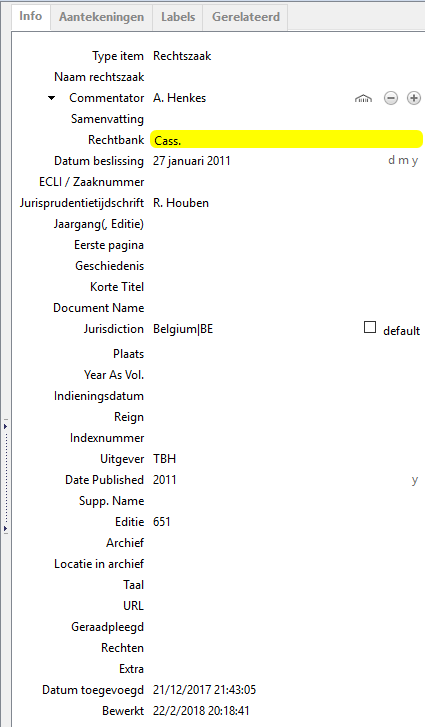
\includegraphics[scale=0.5]{v-en-a/Manual-fig-4}
\par\end{centering}
\caption{Rechtszaak weergave in Juris-M}
\end{figure}


\section{Boeken, tijdschriften, etc..}

Geen bijzonderheden.
\end{document}
